\chapter{Practice: Blink a LED on the XBee from a computer}

In this assignment we will only use two XBees, a protoboard and a LED.
We will not use the Arduino.

Flash the two XBees.
The ``local'' one will be the coordinator and the ``remote'' one, a router.
Use the API mode for the coordinator.
For the remote one, you can use either coordinator, router or end device.
As we are going to interact with the local XBee using the Python library, it is necessary to set the API mode to two (AP=2), as shown in Figure~\ref{fig:changingAPIMode}.

Connect the remote XBee to a protoboard and power it through the USB.
Connect the 5V to the supply voltage bus running along the protoboard.
Finally, connect a LED to bus (long leg) and to the D1 (short leg).

We can blink the remote link by changing the state of the D1 pin from a Python program as in the example code \ref{code:remote-blinking}. Make sure that you have the required XBee Python libraries, available through the link provided in Chapter~\ref{cha:sink-in-server}.\\

\begin{lstlisting} [caption = {This example code alternatively changes a remote pin to up and low to blink an LED.}, language = Python, label = {code:remote-blinking}, numbers = left, escapeinside={@}{@}]

#! /usr/bin/python

from xbee import XBee
import serial
import time

ser = serial.Serial('/dev/ttyUSB0', 9600)
xbee = XBee(ser)

while True:
    try:
        xbee.send('remote_at', 
                  frame_id='A',
                  dest_addr_long='\x00\x00\x00\x00\x00\x00\xFF\xFF',
                  dest_addr='\xFF\xFE',
                  options='\x02',
                  command='D1',
                  parameter='\x05')
          
        time.sleep(1)
        
        xbee.send('remote_at', 
                  frame_id='A',
                  dest_addr_long='\x00\x00\x00\x00\x00\x00\xFF\xFF',
                  dest_addr='\xFF\xFE',
                  options='\x02',
                  command='D1',
                  parameter='\x04')
          
        time.sleep(1)
    except KeyboardInterrupt:
        break

xbee.send('remote_at', 
          frame_id='A',
          dest_addr_long='\x00\x00\x00\x00\x00\x00\xFF\xFF',
          dest_addr='\xFF\xFE',
          options='\x02',
          command='D1',
          parameter='\x05')

ser.close()


\end{lstlisting}

\begin{figure}[htbp]
  \centering
  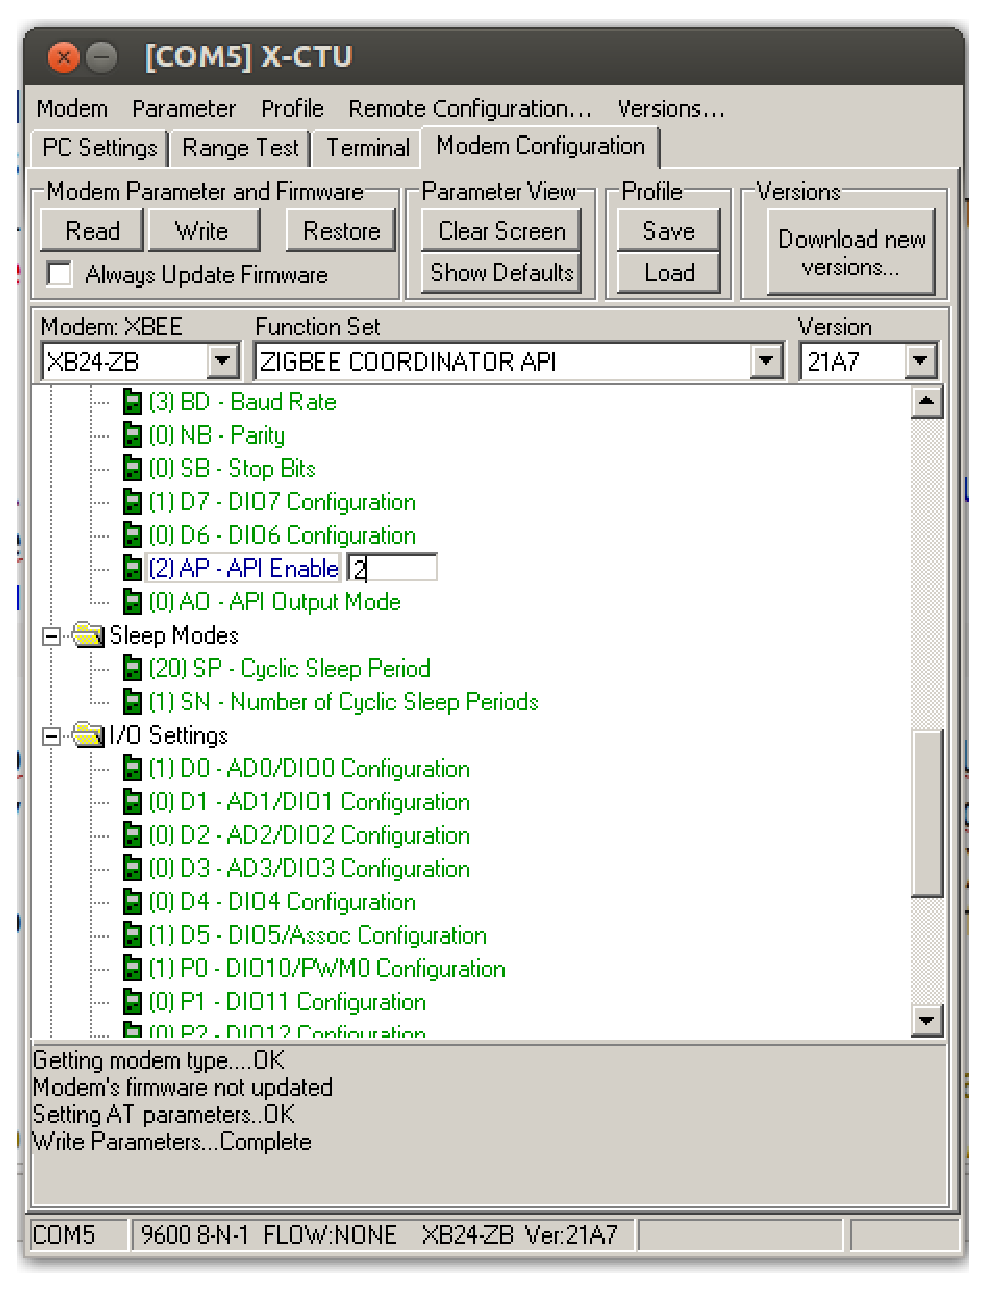
\includegraphics[width=0.85\linewidth]{figures/changingAPIMode.eps}
  \caption{Setting the API mode to 2 (AP=2).}
  \label{fig:changingAPIMode}
\end{figure}

\section{Next steps}
In the example code we use broadcast packets.
Try to blink LEDs in three different XBees alternatively. 
During the first second, the first LED is on.
For the second second, the second LED is on.
And the third LED is on for the third second.
To achieve this you will need to use targeted packets with an explicit destination.

We can also implement the ``sunset sensor'' lab using a computer instead of the arduino.
